%!TeX root=../thesis.tex
%("dica" para o editor de texto: este arquivo é parte de um documento maior)
% para saber mais: https://tex.stackexchange.com/q/78101/183146

\chapter{Research Methodology}
\label{chap:research_methodology}
%%%%%%%%%%%%%%%%%%%%%%%%%%%%%%%%%%%%%%%%%%%%%%%%%%%%%%%%%%%%%%%%%%%%%%%%%%%%%%%%

  This chapter presents the methodology to answer the research questions
  described in \cref{chap:introduction}.
  \Cref{sec:methodology_phase_1,sec:methodology_phase_2,sec:methodology_phase_3}
  present the structure summarized in \cref{fig:research_methodology}.
  Finally, \Cref{sec:methodology_results_threats} discusses expected results
  and threats to validity.
  % Afterward, \cref{chap:work_plan} duscuss the timeline for executing it.

  %----------------------------------------------------------------------------%
  \begin{figure}[hb!]
    \centering
    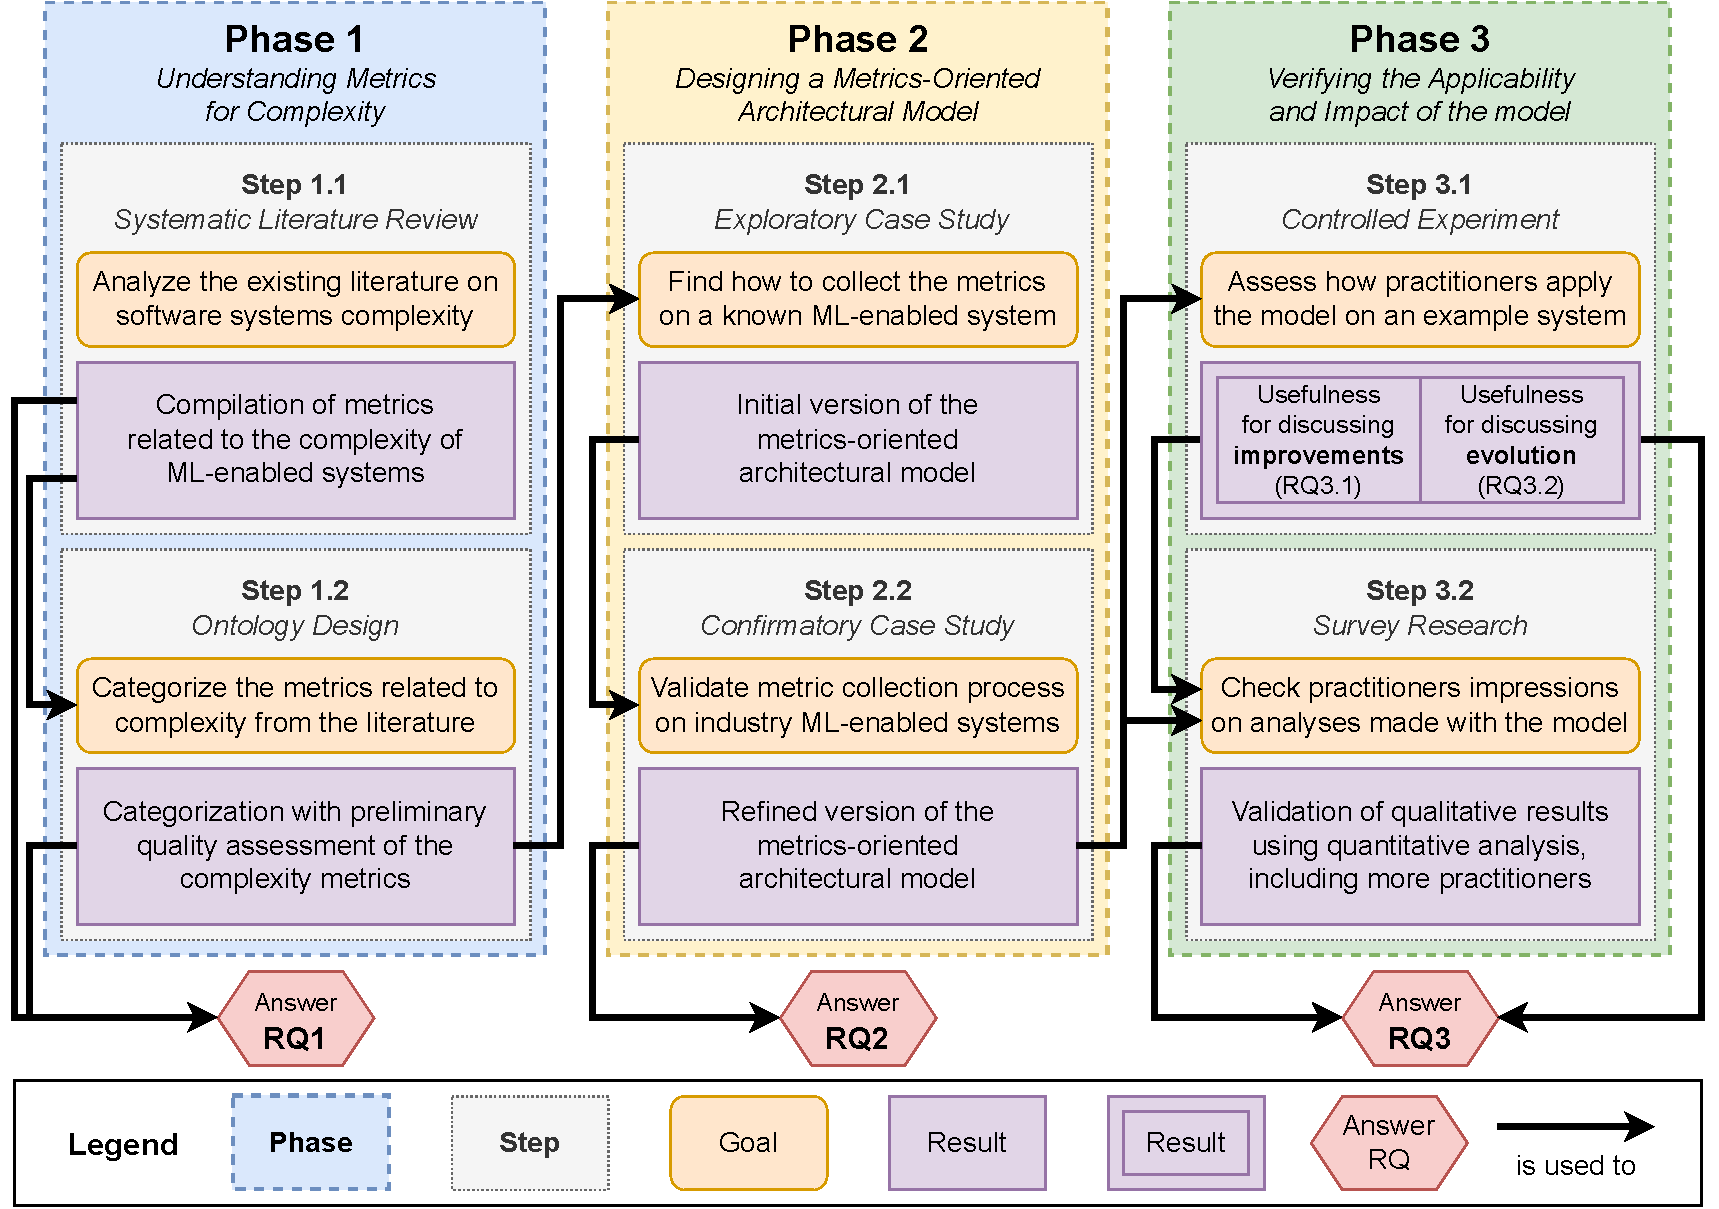
\includegraphics[width=\linewidth]{figures/Methodology.pdf}
    \caption[%
      Research Methodology%
    ]{%
      \emph{Research Methodology}.
      The methodology is divided into three phases. Each phase addresses one
      of the research questions presented in \cref{chap:introduction}. Phases
      are further subdivided into two steps. Each step has a specific goal,
      an expected result, and relies on a research method. Arrows show where
      a result will be used: either to achieve the goal of a later step, or
      to directly answer a research question. This methodology categorizes
      as empirical software engineering~\parencite{Shull2008GuideEngineering},
      with a mixed-method approach.
    }
    \label{fig:research_methodology}
  \end{figure}
  %----------------------------------------------------------------------------%

  \clearpage

  % As an empirical software engineering research, this methodology adopts
  % a \emph{pragmatic stance}~\parencite{Easterbrook2008SelectingEngineering}:
  % any expected results will be more valuable if they can be useful to solve
  % practical problems.
  % It is the authors' belief that ML-enabled systems have
  % great potential to impact society, \emph{if they ever come to production}.
  % In \cref{chap:introduction}, this proposal explored the role of \emph{complexity}
  % in hindering the delivery of ML-enabled systems. Therefore, this research
  % proposes to create a technique and validate its use with practitioners:
  % % to help practitioners handle complexity.
  % a \emph{metrics-oriented architectural model to characterize
  % the complexity of ML-enabled systems}

  \section{Understanding Metrics for Complexity}
  \label{sec:methodology_phase_1}
  \MethodologyPhase
  %%%%%%%%%%%%%%%%%%%%%%%%%%%%%%%%%%%%%%%%%%%%%%%%%%%%%%%%%%%%%%%%%%%%%%%%%%%%%%

  As explored in \cref{chap:ml_enabled_systems}, the current literature
  evidences ML-enabled systems are \emph{complex systems}:
  they are made of multiple components orchestrated to create a larger whole%
  ~\parencite{Benton2020MachineApplications,Chadli2024TheStudy,
  Kreuzberger2023MachineArchitecture,Lwakatare2020Large-ScaleSolutions,
  Steidl2023ThePractice,Tamburri2020SustainableChallenges,Tang2021AnSystems},
  which influence each other in expected%
  ~\parencite{John2021TowardsModel,Serban2021PracticesApplications,
  Wan2021HowPractices}
  and unexpected ways%
  ~\parencite{Sculley2015HiddenSystems,Tang2021AnSystems}.
  The first phase of this research focuses on~\cref{rq:1},
  introduced in~\cref{chap:introduction}, which reads as follows:
  
  % Although there is an understanding of different factors that influence this
  % complexity~\parencite{Benton2020MachineApplications,Diaz-De-Arcaya2023ASurvey,
  % Wan2021HowPractices} -- such as volume of data, distributed processing, etc.
  % -- it remains a challenge to quantify it.

  %----------------------------------------------------------------------------%
  \begin{revisitresearchquestion}{1}
      What are the measurable dimensions of complexity in
      the architecture of ML-enabled systems?
  \end{revisitresearchquestion}
  %----------------------------------------------------------------------------%

  To answer \cref{rq:1}, this research will start studying
  \emph{the complexity of software systems} and \emph{metrics}.
  For that, \cref{phase:1} has been divided into two steps, whose goals are:
  %----------------------------------------------------------------------------%
  \begin{enumerate}[label=\theMethPhase.\arabic*.]
      \item to analyze the existing literature on software systems complexity; and
            % \MethodologyStep
      \item to categorize the metrics related to complexity from the literature.
            % \MethodologyStep
  \end{enumerate}
  %----------------------------------------------------------------------------%
  The following sections detail the proposed methods to achieve these goals.%
  ~\Cref{fig:research_methodology} illustrates the connections between this
  phase and the subsequent ones.

  \subsection{Systematic Literature Review}
  \MethodologyStep
  %%%%%%%%%%%%%%%%%%%%%%%%%%%%%%%%%%%%%%%%%%%%%%%%%%%%%%%%%%%%%%%%%%%%%%%%%%%%%%

  % \Cref{step:1.1} can be accomplished via a \emph{Multivocal Literature Review}
  % (MLR)~\parencite{Garousi2016TheLiterature}, a type of \emph{Systematic
  % Literature Review} (SLR)~\parencite{Kitchenham2012SystematicEngineering}
  % that surveys two sources: the traditional peer-reviewed academic literature
  % -- known as ``white'' -- and the non-published industry literature
  % -- known as ``gray''~\parencite{Garousi2020BenefittingResearch}.
  % An MLR is particularly appropriate when an SLR does not suffice.
  % Considering \cref{rq:1}, 
  
  \Cref{step:1.1} can be accomplished via a \emph{Systematic Literature Review}
  (SLR)~\parencite{Kitchenham2012SystematicEngineering}, a type of secondary
  study -- a study of studies~\parencite{Garousi2020BenefittingResearch} --
  that surveys the peer-reviewed academic literature. To compile the current
  knowledge about a subject, the SLR proceeds as follows.
  First, it starts with a keyword-based search into established knowledge
  bases~\parencite{Kitchenham2012SystematicEngineering}, which index
  academic conferences and journals.
  Then, it complements these results via snowballing%
  ~\parencite{Jalali2012SystematicSnowballing}, where more papers may be
  found in the references of the initial pool.
  Then, it filters the papers in multiple successive rounds, according to
  predefined inclusion and exclusion criteria%
  ~\parencite{Kitchenham2012SystematicEngineering}.
  Finally, the resulting set can be analyzed for relevant data.
  % This workflow is reproducible, thus allowing other researchers to reach
  % similar results.
  % This well-defined workflow allows other researchers to reproduce the
  % survey results
  % allowing other researchers to get to the same results.

  Making an SLR ensures a reproducible way to analyze the literature,
  as it is the goal of \cref{step:1.1}. Initially, the SLR will focus on
  finding references about \emph{complexity metrics}, i.e., metrics that
  were created to measure some aspect of complexity. On the one hand,
  this subject has been thoroughly explored by the software engineering
  literature~\parencite{Fenton2014SoftwareEdition,Tu2009TheMetrics}.
  On the other hand, ML-enabled systems have their data and model dimensions%
  ~\parencite{Alves2024PracticesReview,Sato2019ContinuousLearning},
  whose complexity reflects into code, but goes beyond it%
  ~\parencite{ElAlaoui2019BigApproaches,Polancic2017ComplexityReview}.
  Therefore, characterizing the complexity of ML-enabled systems will
  require looking into more metrics than for traditional software-based
  systems.

  \subsection{Ontology Design}
  \MethodologyStep
  %%%%%%%%%%%%%%%%%%%%%%%%%%%%%%%%%%%%%%%%%%%%%%%%%%%%%%%%%%%%%%%%%%%%%%%%%%%%%%

  % In turn, an MLR repeats the same workflow, but it also considers
  % non-peer-reviewed primary sources -- with different degrees of reliability
  % -- found with a general-purpose search engine.

  \Cref{step:1.2} can be accomplished via \emph{ontology design}%
  ~\parencite{Iqbal2013AnReview,NoyOntologyOntology}. An ontology
  is the structure behind a knowledge base, including \emph{classes},
  \emph{properties}, and \emph{restrictions}~\parencite{NoyOntologyOntology}.
  To design an ontology that describes a subject, the process is as follows.
  First, all the relevant terminology on the domain is compiled. Then,
  domain concepts are divided into classes, which may have hierarchical
  relationships between them. Then, all properties associated to each
  class are defined, with their respective value restrictions. Finally,
  a knowledge base can be created by defining instances of the classes,
  which will be composed of properties that respect the restrictions.

  Making an ontology results in a well-defined categorization of the metrics,
  as it is the goal of \cref{step:1.2}. The ontology will focus on describing
  different \emph{types} of metrics~\parencite{Fenton2014SoftwareEdition},
  as well as possible \emph{quality attributes} associated with them%
  ~\parencite{Latva-Koivisto2001FindingModels}. Some properties will be
  related to the \emph{applicability} of the metrics, which will be explored
  only on~\cref{phase:2}. Therefore, the knowledge base will be fully complete
  only by the end of the research.

  \section{Designing a Metrics-Oriented Architectural Model}
  \label{sec:methodology_phase_3}
  \MethodologyPhase
  %%%%%%%%%%%%%%%%%%%%%%%%%%%%%%%%%%%%%%%%%%%%%%%%%%%%%%%%%%%%%%%%%%%%%%%%%%%%%%

  \Cref{phase:1} will result in an overview of the state of the art about
  complexity metrics related to ML-enabled systems. However, as explored in%
  ~\cref{chap:ml_enabled_systems}, these systems have intricate architectures,
  which evolve according to three axes of change: code, model, and data
  ~\parencite{Alves2024PracticesReview,Sato2019ContinuousLearning}.
  The second phase of this research focuses on~\cref{rq:2}, introduced in%
  ~\cref{chap:introduction}, which reads as follows:
  %----------------------------------------------------------------------------%
  \begin{revisitresearchquestion}{2}
    How can complexity metrics be operationalized over
    the architecture of ML-enabled systems?
  \end{revisitresearchquestion}
  %----------------------------------------------------------------------------%

  To answer \cref{rq:2}, this research will focus on selecting a subset of the
  metrics from \cref{phase:1} to design a \emph{metrics-oriented
  architectural model to characterize the complexity of ML-enabled systems}.
  For that, \cref{phase:2} has been divided into two steps, whose goals are:
  %----------------------------------------------------------------------------%
  \begin{enumerate}[label=\theMethPhase.\arabic*.]
      \item to find how to collect the metrics on a known ML-enabled system; and
            % \MethodologyStep
      \item to validate the metric collection process on industry ML-enabled systems.
            % \MethodologyStep
  \end{enumerate}
  %----------------------------------------------------------------------------%
  The following sections detail the proposed methods to achieve these goals.%
  ~\Cref{fig:research_methodology} illustrates the connections between this
  phase and the surrounding ones.

  \subsection{Exploratory Case Study}
  \MethodologyStep
  %%%%%%%%%%%%%%%%%%%%%%%%%%%%%%%%%%%%%%%%%%%%%%%%%%%%%%%%%%%%%%%%%%%%%%%%%%%%%%

  \Cref{step:2.1} can be accomplished via an \emph{exploratory study case}%
  ~\parencite{Easterbrook2008SelectingEngineering}, whose goal is to 
  derive new hypothesis and build theories about a phenomenon. At its core,
  an exploratory case study requires a \emph{study proposition}%
  ~\parencite{Easterbrook2008SelectingEngineering}, which defines:
    what the study aims to achieve,
    which cases will be considered, and
    what types of data will be collected.
  Results come from analyzing the data. However, case studies apply
  \emph{purposive sampling}~\parencite{Easterbrook2008SelectingEngineering},
  where cases are chosen according to their relevance for the study.
  Therefore, great care must be taken to generalize results.

  Making an exploratory case study provides a framework to propose an answer
  to~\cref{rq:2}. The exploratory case study will have the following
  study proposition: \emph{``What is a process to operationalize the
  collection of complexity metrics on an ML-enabled system?''}, as it is
  the goal of \cref{step:2.1}. To achieve that, it will rely on a
  \emph{typical case}~\parencite{Easterbrook2008SelectingEngineering}:
  the SPIRA ML-enabled system, previously introduced
  in~\cref{chap:the_spira_system}.

  SPIRA is an open-source project, architected at the beginning of
  this PhD~\parencite{Ferreira2022SPIRA:Detection}. As explained in
  \cref{chap:the_spira_system}, it contains all the basic components of
  the reference architecture from \cref{chap:ml_enabled_systems}.
  The familiarity with the codebase should allow the authors to focus
  on operationalizing the metric collection rather than learning how the
  project works. The goal is twofold:
    document \emph{the process of metric collection},
    to achieve the study proposition; and
    determine \emph{the quality attributes of the metrics},
    to refine the ontology made on \cref{step:1.2}.
  By choosing which metrics are worth collecting, and documenting
  the requirements to collect them, the result will be the initial version
  of the \emph{metrics-oriented architectural model}.

  \subsection{Confirmatory Case Study}
  \MethodologyStep
  %%%%%%%%%%%%%%%%%%%%%%%%%%%%%%%%%%%%%%%%%%%%%%%%%%%%%%%%%%%%%%%%%%%%%%%%%%%%%%

  \Cref{step:2.2} can be accomplished via a \emph{confirmatory case study}%
  ~\parencite{Easterbrook2008SelectingEngineering}, whose goal is to 
  test and validate existing theories about a phenomenon. Similarly,
  a confirmatory case study requires a \emph{study proposition}%
  ~\parencite{Easterbrook2008SelectingEngineering}, which defines:
    what the study aims to achieve,
    which cases will be considered, and
    what types of data will be collected.
  Results come from analyzing the data. These case studies can be seen as a
  \emph{replication}~\parencite{Easterbrook2008SelectingEngineering}:
  they either expect the same results -- \emph{literal replications} --
  or predict contrasting results -- \emph{theoretical replications}.
  Regardless, designing multiple case studies offers greater validity
  to results~\parencite{Easterbrook2008SelectingEngineering}.

  Making a confirmatory case study provides a framework to validate the
  proposed answer to~\cref{rq:2}. The confirmatory case study will repeat
  the same study proposition: \emph{``What is a process to operationalize
  the collection of complexity metrics on an ML-enabled system?''}, as it
  is the goal of \cref{step:2.2}. To achieve that, it will rely on
  industry partners of the Jheronimus Academy of Data Science (JADS).

  Production ML-enabled systems can have various architectures, with
  different combinations of components. The diversity of codebases
  should allow the researchers to validate the robustness of the
  metric collection process. Two types of data will be revisited:
    \emph{the process of metric collection},
    to achieve the study proposition; and
    \emph{the quality attributes of the metrics},
    to refine the ontology made on \cref{step:1.2}.
  By reviewing which metrics are worth collecting and the requirements
  to collect them, the result will be a refined version of the
  \emph{metrics-oriented architectural model}.

  % In principle, all metrics found in%
  % ~\cref{phase:1} should be useful, since by design they will be related
  % to complexity. Moreover, 
  
  % which subset of metrics from~\cref{phase:1}
  % should be used to characterize the complexity of ML-enabled systems.
  
  \section{Verifying Applicability and Impact}
  \label{sec:methodology_phase_2}
  \MethodologyPhase
  %%%%%%%%%%%%%%%%%%%%%%%%%%%%%%%%%%%%%%%%%%%%%%%%%%%%%%%%%%%%%%%%%%%%%%%%%%%%%%

  \Cref{phase:2} will lead to the development of a \emph{metrics-oriented
  architectural model to characterize the complexity of ML-enabled systems}.
  However, following a pragmatic stance~\parencite{Easterbrook2008SelectingEngineering}, 
  the model is valuable if it can be used to help practitioners.
  The third phase of this research focuses on~\cref{rq:3}, introduced in%
  ~\cref{chap:introduction}, which reads as follows:
  %----------------------------------------------------------------------------%
  \begin{revisitresearchquestion}{3}
      How can complexity metrics be used to aid the development,
      operation, and evolution of real-world ML-enabled systems?
  \end{revisitresearchquestion}
  %----------------------------------------------------------------------------%
  
  To answer \cref{rq:3}, this research will investigate \emph{the
  applicability and impact} of the \emph{metrics-oriented architectural model}.
  For that, \cref{phase:3} has been divided into two steps, whose goals are:
  %----------------------------------------------------------------------------%
  \begin{enumerate}[label=\theMethPhase.\arabic*.]
      \item to assess how practitioners apply the model on an example system, and
            % \MethodologyStep
      \item to check practitioners' impressions on analysis made with the model.
            % \MethodologyStep
  \end{enumerate}
  %----------------------------------------------------------------------------%
  Since the scope of~\cref{rq:3} is very broad, the research will focus on the
  two development tasks described by the subquestions of~\cref{rq:3}:
  %----------------------------------------------------------------------------%
  \begin{revisitresearchquestion}{3.1}
      How can complexity metrics be used to choose between architecture
      proposals for an ML-enabled system?
  \end{revisitresearchquestion}%
  \vspace{-\baselineskip}%
  \begin{revisitresearchquestion}{3.2}
      How can complexity metrics be used to identify refactoring
      opportunities in an ML-enabled systems?
  \end{revisitresearchquestion}
  %----------------------------------------------------------------------------%
  The following sections detail the proposed methods to achieve these goals.
  This phase proposes a \emph{mixed-method approach} to provide generalizable
  results~\parencite{Easterbrook2008SelectingEngineering}.%
  ~\Cref{fig:research_methodology} illustrates the connections between this
  phase and the previous ones.

  \subsection{Controlled Experiment}
  \MethodologyStep
  %%%%%%%%%%%%%%%%%%%%%%%%%%%%%%%%%%%%%%%%%%%%%%%%%%%%%%%%%%%%%%%%%%%%%%%%%%%%%%

  \Cref{step:3.1} can be accomplished via a \emph{controlled experiment}%
  ~\parencite{Easterbrook2008SelectingEngineering}, whose goal is to 
  test a \emph{hypothesis} about of a broad population of individuals.
  % What do we have in an experiment?
  For that, a study has to be designed, containing
  \emph{Independent variables} whose values are manipulated
  to observe causal effects on \emph{dependent variables}.
  Each combination of independent variables set is called
  a \emph{treatment}~\parencite{Easterbrook2008SelectingEngineering}.
  % Hipothesis -> Variables, Theory -> Subjects
  For the study, the hypothesis guides the choice of variables,
  whereas the theory behind it helps to select a target population.
  % Impact of careful sampling
  Since the controlled experiment uses \emph{sampling},
  it must have a well-defined population and a clear process
  to select subjects~\parencite{Easterbrook2008SelectingEngineering}.
  % Consequence: results are generalizable
  This way, researchers can claim results are generalizable.
  % But... What is the main challenge?
  However, the main challenge is to find the right subjects
  while avoiding sample bias.

  Making a controlled experiment will provide the first opportunity
  to understand the applicability of the \emph{metrics-oriented
  architectural model}, as summarized by~\cref{rq:3}. \Cref{step:3.1}
  will test two hypotheses, modeled after~\cref{rq:3.1} and~\cref{rq:3.2}:
  %----------------------------------------------------------------------------%
  \begin{enumerate}[label=H\arabic*.]
    \item Do complexity metrics help practitioners \emph{choose between
          architectural proposals} of an ML-enabled system?
          \label{it:ce_hypothesis_1}
    \item Do complexity metrics help practitioners \emph{identify
          refactoring opportunities} in an ML-enabled system?
          \label{it:ce_hypothesis_2}
  \end{enumerate}
  %----------------------------------------------------------------------------%
  The independent variable will be \emph{access to the metrics provided by
  the metrics-oriented architectural model}, with two treatments: \emph{yes}
  or \emph{no}. The dependent variables will be:
  %----------------------------------------------------------------------------%
  \begin{enumerate}[label=V\arabic*.]
    % braces {} around brackets [] otherwise \item interprets it as an argument
    \item {[categorical]} the simplest architecture chosen, and
          \label{it:ce_dependent_variables_1}
    \item {[numerical]} the number of refactoring opportunities found.
          \label{it:ce_dependent_variables_2}
  \end{enumerate}
  %----------------------------------------------------------------------------%

  % How do we get answers about this?
  To test these hypotheses, the study will require a \emph{constructed example}:
  a complete ML-enabled system.
  % What do the example need?
  It should include a set of architectural proposals to discuss its evolution
  -- among one is the simplest -- and contain predefined refactoring
  opportunities in its codebase -- justifiable by metrics.
  % Who are the subjects?
  Subjects should be Machine Learning Engineers (MLEs), who are
  usually responsible for these tasks~\parencite{Burkov2020MachineEngineering,
  Wilson2022MachineAction}. All subjects will have no familiarity with
  the example, but may vary in their level of proficiency in the field.

  % Dealing with bias
  To avoid bias, the study will apply a ``within subjects design''%
  ~\parencite{Easterbrook2008SelectingEngineering}: each subject will
  analyze the constructed example twice -- first \emph{without metrics},
  then \emph{with metrics}. This introduces a cofounding factor: subjects
  will know more about the example after each treatment. Although this
  \emph{learning effect} is undesirable, it is also realistic:
  metrics of a system are usually collected by its own developers%
  ~\parencite{Fenton2014SoftwareEdition}.
  % Expected result
  Therefore, the controlled experiment will be able to assess if the
  \emph{metrics-oriented architectural model} has the expected impact.

  \subsection{Survey Research}
  \MethodologyStep
  %%%%%%%%%%%%%%%%%%%%%%%%%%%%%%%%%%%%%%%%%%%%%%%%%%%%%%%%%%%%%%%%%%%%%%%%%%%%%%

  \Cref{step:3.2} can be accomplished via a \emph{survey research}%
  ~\parencite{Easterbrook2008SelectingEngineering}, whose goal is to
  make an \emph{inquiry} about a broad population of individuals.
  % What do we have in a survey?
  For that, a questionnaire survey has to be designed, containing
  \emph{demographic questions} about its participants and
  \emph{subjective questions} about the inquiry%
  ~\parencite{Easterbrook2008SelectingEngineering}.
  % Inquiry -> Questions, Theory -> Participants
  For the questionnaire, the inquiry guides the choice of questions,
  whereas the theory behind it helps to select a target population.
  % Impact of careful sampling
  Since the survey research uses \emph{sampling},
  it must have a well-defined target population and a clear process
  to reach participants~\parencite{Easterbrook2008SelectingEngineering}.
  % Consequence: results are generalizable
  This way, researchers can claim results are generalizable.
  % But... What is the main challenge?
  However, the main challenge is to get high response rates
  while avoiding sample bias.

  Making a survey research will provide an opportunity to validate
  the applicability of the \emph{metrics-oriented architectural model},
  as summarized by~\cref{rq:3}. \Cref{step:3.2} will make two inquiries,
  modeled after~\cref{rq:3.1} and~\cref{rq:3.2}:
  %----------------------------------------------------------------------------%
  \begin{enumerate}[label=Q\arabic*.]
    \item Do complexity metrics help practitioners understand \emph{why
          an architectural proposal was chosen} for an ML-enabled system?
          \label{it:sr_question_1}
    \item Do complexity metrics help practitioners understand \emph{why
          a refactoring opportunity was found} in an ML-enabled system?
          \label{it:sr_question_2}
  \end{enumerate}
  %----------------------------------------------------------------------------%

  % How do we get answers about this?
  To make these inquiries, the questionnaire will require a set of
  \emph{constructed scenarios}: snippets of ML-enabled systems.
  % What does the scenarios need?
  They should include a set of discussions about architectural proposals
  -- describing the rationale for a premade metrics-based choice --
  and showcase refactoring opportunities in a codebase -- justified by metrics.
  % Who are the subjects?
  Participants should be Machine Learning Engineers (MLEs), who are
  usually responsible for these tasks~\parencite{Burkov2020MachineEngineering,
  Wilson2022MachineAction}. All participants will have no familiarity with
  the scenarios, but may vary in their level of proficiency in the field.

  % Dealing with bias
  To avoid bias, the questionnaire will collect demographic data to account
  for participants' professional experience during the analysis of results.
  Moreover, it will contain multiple scenarios for each inquiry.
  % Expected result
  Therefore, the survey research will be able to assess if the
  \emph{metrics-oriented architectural model} has the expected impact.
  % Expected result
  Finally, it will also provide a quantitative validation to the qualitative
  results found in \cref{step:3.1}.

  % \clearpage

  \section{Expected Results and Threats to Validity}
  \label{sec:methodology_results_threats}
  %%%%%%%%%%%%%%%%%%%%%%%%%%%%%%%%%%%%%%%%%%%%%%%%%%%%%%%%%%%%%%%%%%%%%%%%%%%%%%

  % This section discusses expected results and possible threats to validity after
  % executing the research methodology summarized in \cref{fig:research_methodology}.

  As an empirical software engineering research, this methodology adopts
  a \emph{pragmatic stance}~\parencite{Easterbrook2008SelectingEngineering}:
  any expected results will be more valuable if they can be useful to solve
  practical problems. Therefore, the methodology adopted a \emph{mixed-method
  approach}~\parencite{Easterbrook2008SelectingEngineering} to create a
  technique and validate its use with practitioners.
  
  % It is the authors' belief that ML-enabled systems have
  % great potential to impact society, \emph{if they ever come to production}.
  % In \cref{chap:introduction}, this proposal explored the role of \emph{complexity}
  % in hindering the delivery of ML-enabled systems. Therefore, this research
  % proposes to create a technique to help practitioners handle complexity.
  % a \emph{metrics-oriented architectural model to characterize
  % the complexity of ML-enabled systems}

  To ensure the methodology is scientifically sound, it is important to discuss
  its limitations. According to \citeauthor{Easterbrook2008SelectingEngineering}%
  ~\parencite{Easterbrook2008SelectingEngineering}, an empirical software
  engineering research may have four types of threats to validity:
  %----------------------------------------------------------------------------%
  \begin{itemize}
    \item \emph{construct validity},
          if a study can measure what it proposed to measure;
          \label{it:threat_construct_validity}
    \item \emph{internal validity},
          if a study can produce the results it reported;
          \label{it:threat_internal_validity}
    \item \emph{external validity},
          if a study can be generalized to other contexts; and
          \label{it:threat_external_validity}
    \item \emph{conclusion},
          if a study can be replicated by other researchers.
          \label{it:threat_conclusion}
  \end{itemize}
  %----------------------------------------------------------------------------%

  The remaining of this section is divided as follows: for each phase of the
  methodology summarized in \cref{fig:research_methodology}, it highlights the
  main expected result, the potential threats to validity, and the proposed
  solutions to contain these threats.
  % details the expected results of each phase of

  %----------------------------------------------------------------------------%
  \begin{expectedresult}
    The state of the art about complexity metrics for ML-enabled systems.
  \end{expectedresult}
  %----------------------------------------------------------------------------%

  \Cref{phase:1} is mostly subject to \emph{internal} and \emph{conclusion}
  threats to validity. \Cref{step:1.1} leads to an internal threat because
  the SLR depends on the data provided by knowledge bases. \Cref{step:1.2}
  leads to a conclusion threat because it produces an ontology -- whose
  design is a subjective process by itself -- based on the data gathered
  on the previous step.

  To contain the internal threat, this research will produce an SLR
  based on the most established publication databases in Computer Science,
  including ACM, IEEE, Elsevier, and Scopus. To contain the conclusion threat,
  it will follow well-established guidelines available in the literature,
  both for the SLR~\parencite{Kitchenham2012SystematicEngineering} and for
  the ontology~\parencite{NoyOntologyOntology}. By documenting the process
  thoroughly, the results from~\cref{phase:1} should be reliable for the
  next phases.

  %----------------------------------------------------------------------------%
  \begin{expectedresult}
    An academic- and industry-based case study on complexity metrics for
    ML-enabled systems.
  \end{expectedresult}
  %----------------------------------------------------------------------------%

  \Cref{phase:2} is mostly subject to \emph{external} and \emph{conclusion}
  threats to validity. Both \cref{step:2.1,step:2.2} are case studies that
  will incrementally result in the \emph{metrics-oriented architectural model
  to characterize the complexity of ML-enabled systems}. They will be based
  on the analysis of existing ML-enabled systems: the SPIRA system for
  \cref{step:2.1}, and production systems from industry partners for
  \cref{step:2.1}. The choice of systems included in the case studies
  leads to the external threat, whereas the selection of metrics that
  compose the model leads to the conclusion threat.

  To contain the external threat, this research will define inclusion and
  exclusion criteria to accept an ML-enabled system in the case study.
  As it was considered for SPIRA, any production system from an industry
  partner will be considered only if they contain key components of the
  reference architecture explored in~\cref{chap:ml_enabled_systems}.
  To contain the conclusion threat, \cref{phase:2} was designed to have
  first an exploratory and then a confirmatory case study.
  The \emph{metrics-oriented architectural model} will be developed
  iteratively, ensuring its metric collection process is tested in
  multiple systems. By creating a reliable model, the results from
  \cref{phase:2} can be confidently used in the next phase.

  %----------------------------------------------------------------------------%
  \begin{expectedresult}
    A mixed-method approach to assess the impact of complexity metrics
    in development tasks of ML-enabled systems.
  \end{expectedresult}
  %----------------------------------------------------------------------------%
  
  \Cref{phase:3} is mostly subject to \emph{construct} and \emph{external}
  threats to validity. \Cref{step:3.1} leads to a construct threat because
  it will use a \emph{constructed example} in its controlled experiment,
  whereas \cref{step:3.2} will use \emph{constructed scenarios} in its
  survey research. Moreover, both \cref{step:3.1,step:3.2} lead
  to an external threat because they depend on sampling a population of
  practitioners. Results can be very different depending on who joins
  the studies.

  To contain the construct threat, this research will use \emph{peer review}
  with collaborators to check the constructed examples. Moreover, it will
  execute alpha tests on both steps, discarding results to collect feedback
  and refine the study. To contain the external threat, this research will
  take advantage that the authors are active members of the Software Engineering
  and Machine Learning Engineering communities. With a large contact network,
  the studies can reach more practitioners, thus decreasing sampling bias.
  By including a significant number of people, the results from \cref{phase:3}
  can provide valuable insight for practitioners in the field.

  Finally, each result of this methodology has the potential to generate
  publications. Since this is an empirical software engineering research%
  ~\parencite{Shull2008GuideEngineering}, they may be submitted to high-impact
  conferences and journals. In particular, some venues provided many references
  used during this research. Here is a list of venues to which the authors
  plan to submit:
  %----------------------------------------------------------------------------%
  \begin{itemize}
    \item International Conference on AI Engineering (CAIN)%
          ~\parencite{   
            Granlund2021MLOpsCases,
            Lewis2021CharacterizingSystems,
            Makinen2021WhoHelp,
            Nahar2023APractitioners,
            Serban2021PracticesApplications,
          }.
    \item International Conference on Software Engineering (ICSE)%
          ~\parencite{
            Amershi2019SoftwareStudy,
            Kolltveit2022OperationalizingReview,
            Nahar2021MoreProjects,
          }.
    \item Journal of Systems and Software%
          ~\parencite{
            Foidl2024DataDevelopers,
            Giray2021AChallenges,
            Steidl2023ThePractice,
          }.
    \item ACM Computing Surveys%
          ~\parencite{
            Diaz-De-Arcaya2023ASurvey,
            Paleyes2022ChallengesStudies,
          }.
    \item ACM Transactions on Software Engineering and Methodology (TOSEM)%
          ~\parencite{Martinez-Fernandez2022SoftwareSurvey}.
  \end{itemize}
  %----------------------------------------------------------------------------%